% Relatório do projeto — versão LaTeX (pdfLaTeX).
% Autossuficiente: zipe esta pasta e faça upload no Overleaf que compila direto.
\documentclass[12pt,a4paper]{article}

\usepackage[utf8]{inputenc}
\usepackage[T1]{fontenc}
\usepackage[brazil]{babel}
\usepackage[margin=2.5cm]{geometry}
\usepackage{graphicx}
\usepackage{booktabs}
\usepackage{tabularx}
\usepackage{amssymb}
\usepackage{enumitem}
\usepackage[hidelinks]{hyperref}

\graphicspath{{figuras/}}
\setlength{\parskip}{0.5em}
\setlength{\parindent}{0pt}

\title{Porteiro Eletrônico Inteligente\\[2pt]
\large Sistema de Segurança com Vídeo e Alerta}
\author{%
Douglas Monteiro Almeida Souza — NUSP 10748048 \\
Guilherme Junji Tutiya — NUSP 14576065 \\
Henrique Maruiti — NUSP 12610243}
\date{PCS3732 — Laboratório de Processadores \\
Entrega: Semana 2 — Servidor de vídeo / Streaming da câmera (RF1)}

\begin{document}
\maketitle

\section{Motivação / Justificativa}

Sistemas de portaria e monitoramento por vídeo são cada vez mais comuns em
condomínios, comércios e instituições, mas soluções comerciais completas
costumam ter custo elevado e serem fechadas (difíceis de adaptar). O objetivo
deste projeto é demonstrar, com hardware de baixo custo (Raspberry Pi + câmera),
que é possível montar um \textbf{porteiro eletrônico} que transmite vídeo em
tempo real para um posto de monitoramento e permite ao vigia acionar um
\textbf{alerta de emergência} por um botão físico.

A ideia central é a de um sistema de vigilância simples: uma câmera controlada
por um Raspberry Pi, um computador central que exibe o vídeo em \textit{streaming}
e um botão que dispara uma notificação (por exemplo, acionar a polícia) ao
identificar algo suspeito.

Projetos e referências similares:
\begin{itemize}[nosep]
  \item Streaming de vídeo com ESP32-CAM via Wi-Fi (tutorial de referência):
        \url{https://www.youtube.com/watch?v=YG08Sl1JbQw}
  \item Transmissão MJPEG (\texttt{multipart/x-mixed-replace}) como técnica de
        baixo custo de latência para vídeo em rede local.
\end{itemize}

\section{Objetivos}

\textbf{Objetivo geral:} desenvolver um sistema de segurança que simula um
porteiro eletrônico, com transmissão de vídeo em tempo real para um computador
central e acionamento de alerta de emergência por botão físico.

\textbf{Objetivos específicos:}
\begin{itemize}[nosep]
  \item Transmitir vídeo da câmera da borda para o central em tempo real (MJPEG).
  \item Permitir ajuste da qualidade da câmera via software, remotamente.
  \item Detectar o acionamento de um botão físico e disparar uma notificação de
        emergência.
  \item Monitorar e controlar a latência da transmissão.
  \item Garantir disponibilidade do sistema durante a operação (reconexão
        automática).
  \item Estruturar o código em camadas de baixo acoplamento, facilitando
        manutenção e troca de hardware.
\end{itemize}

\section{Requisitos Funcionais}

\begin{tabularx}{\textwidth}{l X}
\toprule
\textbf{ID} & \textbf{Requisito} \\
\midrule
RF1 & Câmera que transmite vídeo em tempo real. \\
RF2 & Botão físico que aciona um alarme/notificação de emergência. \\
RF3 & Ajuste da qualidade da câmera via software. \\
\bottomrule
\end{tabularx}

\section{Requisitos Não Funcionais}

\begin{tabularx}{\textwidth}{l X}
\toprule
\textbf{ID} & \textbf{Requisito} \\
\midrule
RNF1 & Controle de latência da câmera. \\
RNF2 & Disponibilidade de pelo menos 95\% do tempo de operação. \\
RNF3 & Código com padrões que facilitam alterações futuras (baixo acoplamento). \\
\bottomrule
\end{tabularx}

\section{Diagramas da Arquitetura}

As fontes editáveis dos diagramas estão no repositório em \texttt{docs/diagramas/}
(formato D2); as figuras renderizadas, em \texttt{docs/figuras/} (reproduzidas
adiante).

\section{Arquitetura Física}

A solução usa uma arquitetura cliente-servidor em três camadas, com baixo
acoplamento entre elas:
\begin{enumerate}[nosep]
  \item \textbf{Borda (Edge)} — Raspberry Pi 3B+ com a câmera e o botão de alarme.
        Roda o firmware que captura imagem e serve o vídeo, além de ler o botão
        via GPIO.
  \item \textbf{Rede Wi-Fi 802.11} — canal de comunicação entre borda e central.
        Na Semana 2 adotou-se o Raspberry Pi em \textbf{modo Access Point}
        (hotspot próprio, via \texttt{nmcli}): o central conecta-se diretamente ao
        Wi-Fi do Pi (IP \textasciitilde{}\texttt{10.42.0.1}), sem roteador nem
        internet. Isso adequa-se a um porteiro local e contorna o \textit{isolamento
        de clientes} comum em redes compartilhadas (ex.: Wi-Fi institucional), que
        impede um dispositivo de alcançar o outro.
  \item \textbf{Computador Central} — recebe o vídeo, exibe a interface de
        monitoramento (Dashboard), mede a latência, permite configurar a câmera e
        trata o alarme.
\end{enumerate}

\begin{figure}[h]
  \centering
  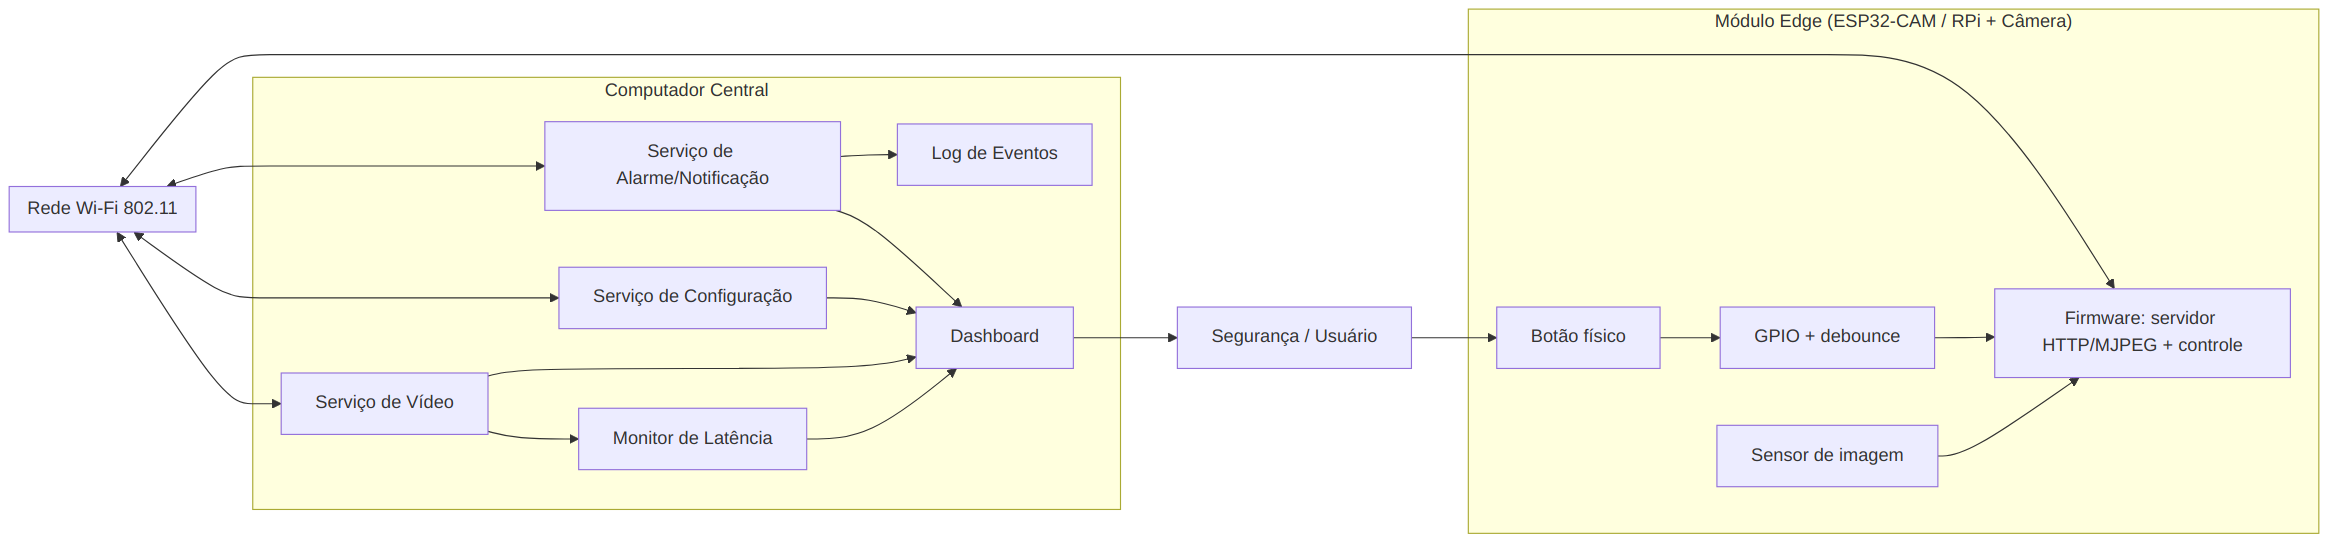
\includegraphics[width=0.9\linewidth]{diagrama_blocos.png}
  \caption{Diagrama de blocos da arquitetura.}
\end{figure}

\textbf{Pendência de hardware (câmera):} a captura de vídeo é parte essencial do
projeto. Ainda é necessário \textbf{confirmar o acesso ao módulo de câmera CSI}
para o Raspberry Pi; caso não esteja disponível, a alternativa é usar uma
\textbf{câmera USB}. Essa decisão altera apenas o backend de captura (ver Seção 7),
não a arquitetura.

\section{Arquitetura de Software}

\textbf{Modelagem estática.} O código é dividido por camada (ver \texttt{src/}):
\begin{itemize}[nosep]
  \item \texttt{src/rpi/camera\_stream.py} — servidor de vídeo da borda
        (\textbf{implementado na Semana 2}: \texttt{GET /} e \texttt{GET /stream}
        MJPEG). A captura fica isolada atrás de uma interface (\texttt{FrameSource}),
        com o backend escolhido automaticamente por \texttt{make\_source()} na ordem
        \texttt{picamera2} (módulo CSI, primário) $\rightarrow$ OpenCV/V4L2 (câmera
        USB, \textit{fallback}) $\rightarrow$ fonte sintética (frames gerados por
        software, para desenvolvimento e teste sem hardware). Assim, a pendência da
        câmera não afeta o restante do sistema (RNF3).
  \item \texttt{src/rpi/alarme.py} — leitura do botão com \texttt{gpiozero.Button}
        e debounce por \texttt{bounce\_time}.
  \item \texttt{src/central/monitor.py} — Dashboard/Serviço de Vídeo, Monitor de
        Latência e Serviço de Alarme.
\end{itemize}

\textbf{Modelagem comportamental.} Dois fluxos principais:
\begin{itemize}[nosep]
  \item \textit{Streaming:} o central abre \texttt{GET /stream} no firmware; a cada
        frame, um JPEG independente é enviado no formato
        \texttt{multipart/x-mixed-replace}, a latência é medida e a imagem é
        atualizada. A qualidade é ajustada por
        \texttt{GET /control?var=quality\&val=X}.
  \item \textit{Alarme:} ao pressionar o botão, a interrupção de GPIO passa por
        debounce (\textasciitilde{}50\,ms) e o firmware envia \texttt{POST /alert}
        ao central. Havendo rede, o central responde \texttt{200 OK} (ACK), dispara
        a notificação e registra em log; em falha de rede, o firmware retransmite
        com \textit{retry} e \textit{backoff}.
\end{itemize}

\begin{figure}[h]
  \centering
  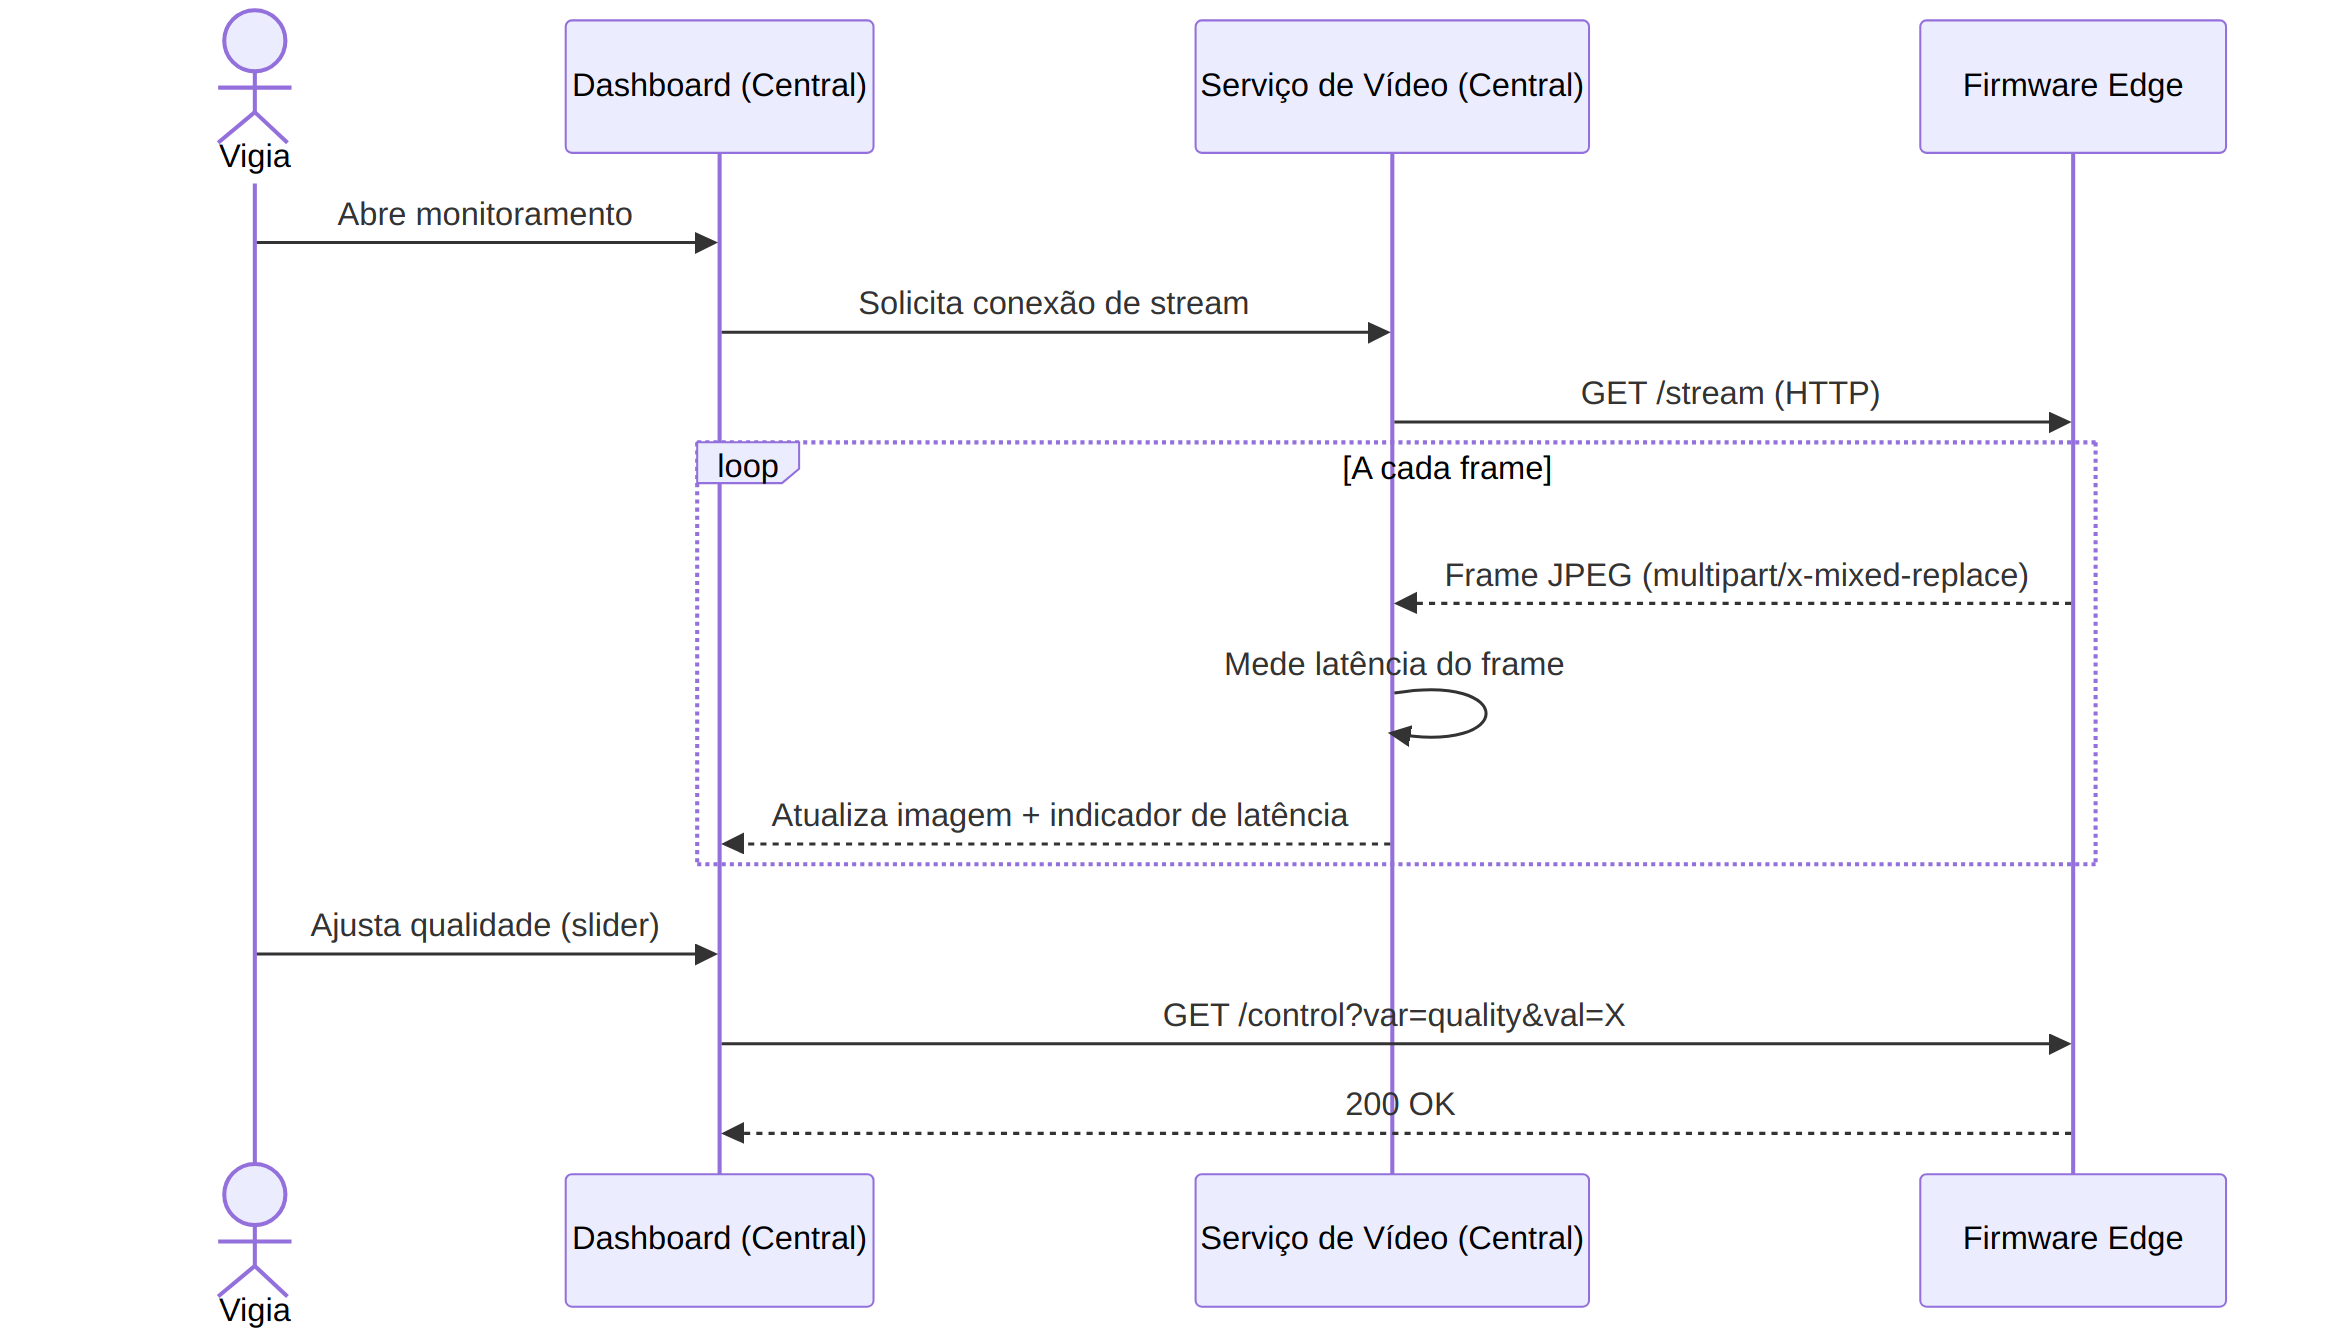
\includegraphics[width=0.85\linewidth]{sequencia_streaming.png}
  \caption{Sequência de streaming.}
\end{figure}

\begin{figure}[h]
  \centering
  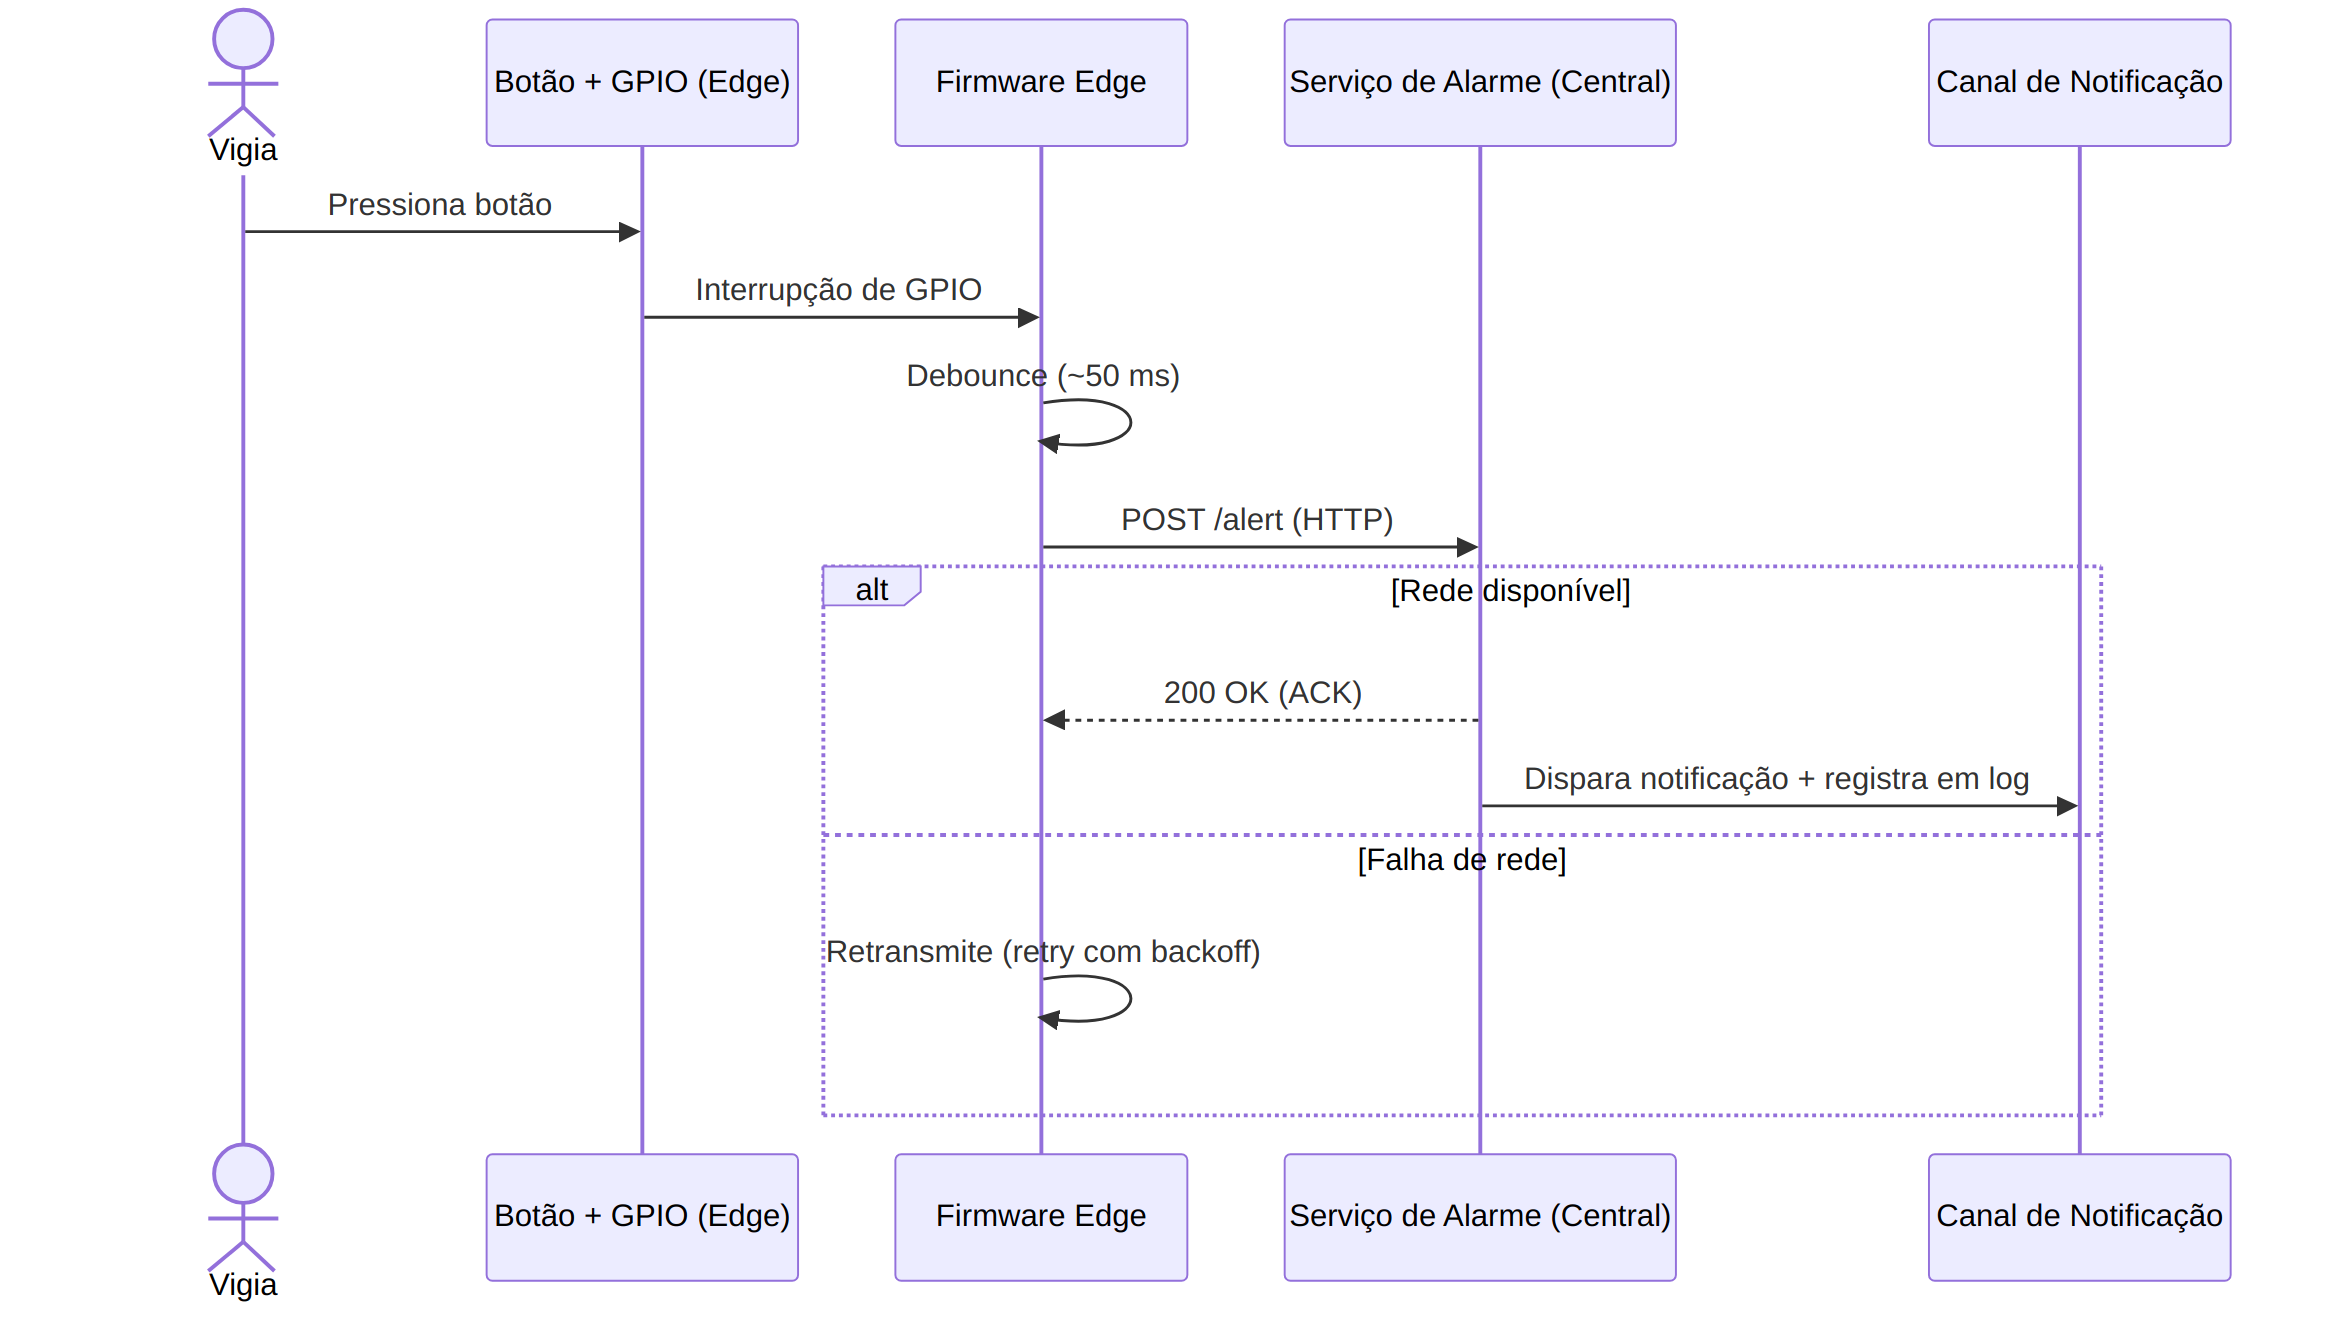
\includegraphics[width=0.85\linewidth]{sequencia_alarme.png}
  \caption{Sequência de alarme.}
\end{figure}

\subsection{Rastreabilidade Requisito $\rightarrow$ Componente}

\begingroup
\small
\begin{tabularx}{\textwidth}{p{2.6cm} p{1.5cm} p{3.3cm} X}
\toprule
\textbf{Requisito} & \textbf{Tipo} & \textbf{Componente(s)} & \textbf{Como é atendido / Justificativa} \\
\midrule
Câmera transmite em tempo real & Funcional & Sensor de imagem + firmware Edge (MJPEG) + Serviço de Vídeo & Streaming \texttt{multipart/x-mixed-replace}: cada frame é independente (sem codec complexo), latência próxima a um período de frame (ZBOTIC, 2026). \\
\addlinespace
Botão aciona alarme & Funcional & GPIO + debounce (Edge), Serviço de Alarme, notificação & Debounce por software evita leituras falsas do contato mecânico (MAKERHERO, 2024); envio HTTP com ACK e retry garante entrega do evento. \\
\addlinespace
Ajuste de qualidade via software & Funcional & Serviço de Configuração + endpoint de controle no Edge & Parâmetro de compressão/resolução alterado remotamente, sem novo firmware — atende ao requisito e reforça manutenibilidade. \\
\addlinespace
Controle de latência & Não funcional & Monitor de Latência + fallback adaptativo no Edge & Mede o tempo de chegada de cada frame; acima do limiar, reduz resolução/qualidade automaticamente. \\
\addlinespace
Disponibilidade $\geq$ 95\% & Não funcional & Reconexão automática de Wi-Fi + retry/backoff + log & Reduz perda de eventos em instabilidades momentâneas de rede; alinhado ao atributo de confiabilidade/disponibilidade da ISO/IEC 25010 (2011). \\
\addlinespace
Código manutenível & Não funcional & Separação em camadas (firmware Edge / serviços Central / interface) & Baixo acoplamento permite trocar hardware (CSI $\leftrightarrow$ USB) ou canal de notificação sem redesenho — princípio de modularidade da ISO/IEC 25010 (2011). \\
\bottomrule
\end{tabularx}
\endgroup

\section{Ferramentas Utilizadas}

\textbf{Linguagens:} Python.

\textbf{Bibliotecas/Frameworks:} \texttt{picamera2} ou OpenCV (captura de imagem),
Flask (servidor HTTP/MJPEG), \texttt{gpiozero} (leitura do botão / GPIO),
\texttt{requests} (envio do alerta). D2 para os diagramas.

\textbf{Hardware:} Raspberry Pi 3B+, câmera (módulo CSI a confirmar, ou câmera
USB), botão físico do kit.

\section{Metodologia de Desenvolvimento}
\begin{itemize}[nosep]
  \item Desenvolvimento incremental ao longo de quatro semanas, com uma
        \textit{Release} por semana no GitHub e o PDF correspondente no Moodle.
  \item Repositório público, com histórico de commits incrementais, uso de
        \textit{branches} e \textit{Pull Requests} (com \textbf{branch única
        \texttt{main}} na entrega final).
  \item Documentação em Markdown, convertida para LaTeX (esta versão).
  \item Documentação do código com \textbf{docstrings no padrão Google}.
  \item Revisão por pares na Semana 2, via GitHub Issues.
\end{itemize}

\section{Testes}

A estratégia de validação e a rastreabilidade entre requisitos e casos de teste
estão em \texttt{tests/rastreabilidade.md}. Na Semana 2 o \textbf{RF1 passou a
resultado obtido}: o stream MJPEG rodou no Raspberry Pi e foi assistido de outro
computador pelo navegador (vídeo contínuo), com o Pi provendo a rede em modo
Access Point. Os demais casos seguem planejados. Os casos de RF2 (evento único
por clique) e RNF3 (backend plugável) são candidatos a \textbf{testes
automatizados} (ponto extra); há uma primeira checagem executável do pipe de
vídeo em \texttt{tests/test\_camera\_stream.py}.

\section{Conclusões (Preliminares)}

Na primeira semana o projeto foi estruturado: repositório organizado,
documentação inicial, diagramas de arquitetura e esqueleto do código em camadas.
A arquitetura em três camadas de baixo acoplamento tende a atender aos requisitos
funcionais (streaming, alarme, ajuste de qualidade) e não funcionais (latência,
disponibilidade, manutenibilidade). Na Semana 2, o servidor de vídeo foi
implementado e o \textbf{RF1 validado em hardware} — a câmera do Pi foi assistida
de outro computador (Pi em modo Access Point) —, confirmando na prática a
viabilidade da captura plugável e do streaming MJPEG.

\textbf{Riscos e dificuldades previstas:} confirmação do módulo de câmera CSI
(com \textit{fallback} para câmera USB) e a latência do MJPEG sob a capacidade do
Raspberry Pi 3B+. \textbf{Próximos passos:} o ajuste de qualidade
(\texttt{GET /control}, RF3) e o fluxo do botão de emergência (RF2), seguindo com
os testes da Seção 10.

\section*{Referências}
\addcontentsline{toc}{section}{Referências}

\begingroup
\setlength{\parskip}{0.7em}

ESPRESSIF SYSTEMS. \textbf{ESP32 Series Datasheet}. Version 4.3. Shanghai:
Espressif Systems, 2023. Disponível em:
\url{https://www.espressif.com/sites/default/files/documentation/esp32_datasheet_en.pdf}.
Acesso em: 18 jun. 2026.

INTERNATIONAL ORGANIZATION FOR STANDARDIZATION. \textbf{ISO/IEC 25010:2011} —
Systems and software engineering — Systems and software Quality Requirements and
Evaluation (SQuaRE) — System and software quality models. Geneva: ISO, 2011.

MAKERHERO. \textbf{Debounce: tratando o efeito bounce de botões e chaves}. 2024.
Disponível em: \url{https://www.makerhero.com/}. Acesso em: 18 jun. 2026.

ZBOTIC. \textbf{Streaming de vídeo MJPEG em sistemas embarcados}. 2026.
\endgroup

\end{document}
